\documentclass[11pt, aspectration=169]{beamer}
\usetheme{Copenhagen}
\usecolortheme{seahorse}
\setbeamertemplate{headline}{}
\usepackage{graphicx} % Required for inserting images
\usepackage{amsmath, amssymb, amsthm}
\usepackage{ragged2e}

\title{Predstavitev 1. domače naloge}
\author{Jaka Gregorc, 23221129}
\date{October 2024}

\begin{document}

\maketitle

\begin{frame}{Kazalo}
\tableofcontents
\end{frame}

\section{Predstavitev prve naloge}
\begin{frame}{Predstavitev prve naloge}
\justifying
V prvi nalogi prebiramo podatke iz \textit{naloga1\_1.txt} tekstovne datoteke. V prvi vrstici vsebuje ime parametra, ki ga prebiramo, kar je v tem primeru čas (time [s]). V drugi vrstici dobimo podatek o številu vrstic in številu podatkov v vsaki vrstici. Imamo 100 vrstic in 1 podatek v vsaki. Torej imamo 100 podatkov o času podanih v sekundah, ki jih moramo uvoziti v \textbf{matlab} in shraniti v vektor. Za uvoz v \textbf{matlab} uporabimo funkcijo \textit{importdata}. Funkciji \textit{importdata} podamo podatke o datoteki, iz katere želimo pobrati podatke(\textit{naloga1\_1.txt}). Na drugem mestu podamo parameter \textit{delimiterIn}, ki funkciji pove kako naj podatke ločimo. Nazadnje še dodamo parameter \textit{headerlinesIn}, ki pa pove koliko vrstic naj spusti preden začne brati dokument. S preprostim ukazom \textit{t = data.data(:, 1)} shranimo časovne podatke v vektor t.
\end{frame}

\section{Graf P(t)}
\begin{frame}{Graf moči v odvisnosti od časa}
Spodaj je izrisan graf \ref{fig:Graf P(t)} moči v odvisnosti od časov, ki smo jih uvozili iz priloženih datotek. Vidimo lahko, da moč s časom eksponentno pada.
\begin{figure}
    \centering
    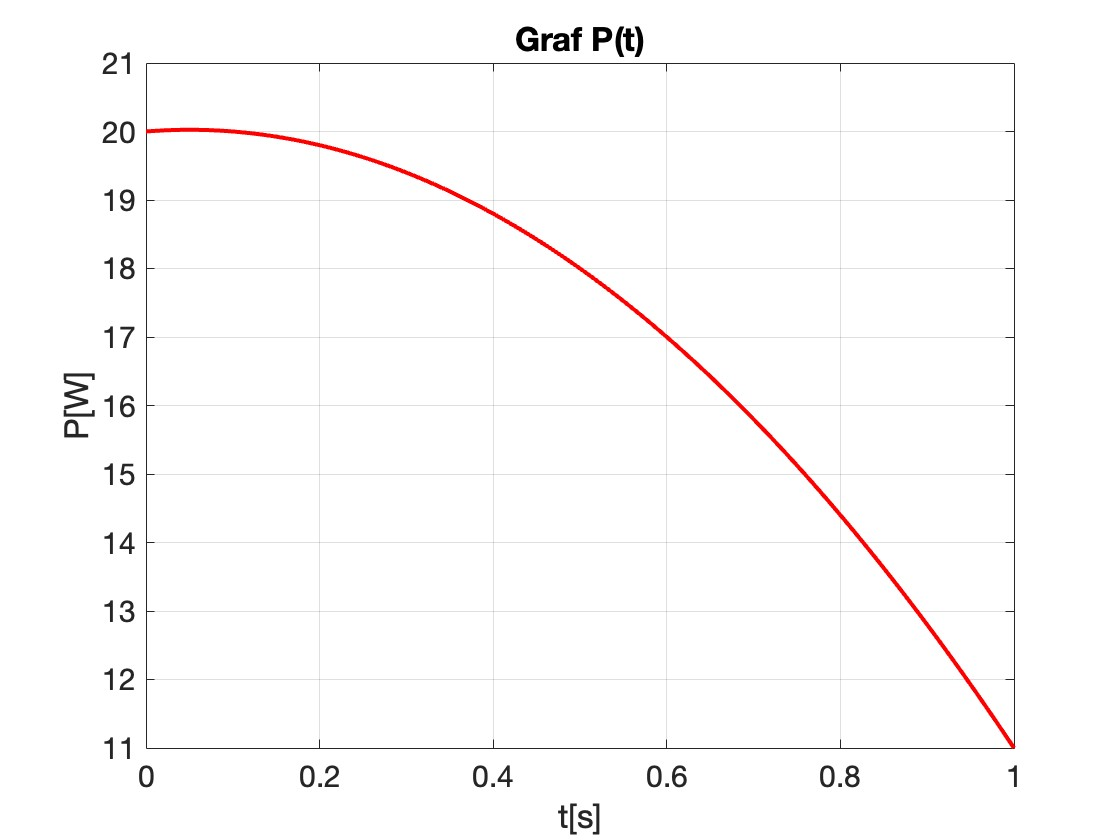
\includegraphics[width=0.65\textwidth]{slike/graf.jpg}
    \caption{Graf P(t) z danimi vhodnimi podatki}
    \label{fig:Graf P(t)}
\end{figure}
    
\end{frame}

\section{Numerično integriranje}
\begin{frame}{Numerično integriranje s trapezno metodo}
Integral smo izračunali s pomočjo built-in funkcije \textit{trapz} in ga primerjali z ročno izračunano vrednostjo integrala glede na teoretično formulo metode.
\begin{block}{Formula za izračun integrala po trapezni metodi}
\small
\[
\int_{a}^{b} f(x) dx = \frac{\Delta x}{2} \left( f(x_0) + 2f(x_1) + 2f(x_2) + \dots + 2f(x_{n-1}) + f(x_n) \right)
\]
\end{block}
\begin{block}{Rešitev našega primera po teoretični formuli}
Torej po zgornji formuli dobimo: 
\[
\int_{t_{min}}^{t_{max}} P(t) dt = \int_{0}^{1} P(t) dt = 17.1665
\]
\end{block}

\end{frame}

\end{document}
